\documentclass[10pt, a4paper]{article}

\usepackage[utf8]{inputenc}
\usepackage[spanish]{babel}
\usepackage{graphicx}
\usepackage{multicol}
\usepackage[usenames,dvipsnames]{color}
\usepackage{amsmath}
\usepackage{verbatim}
\usepackage{footnote}
\usepackage{float}
\usepackage{amsfonts}
\usepackage{hyperref}
\usepackage{framed}
\usepackage{multicol}
\usepackage{pdflscape}

\usepackage{pdfpages}

\usepackage{caratula}

\newcommand{\NonStandardConector}[2] {
	\item \textbf{#1} : #2
}

\materia{Ingeniería de Software II}

\titulo{Trabajo Práctico 2}
\subtitulo{Developing \textsf{in-the-large} - Planificación}
\grupo{Grupo 5 - \emph{El nene está bien}}

\integrante{Martín Alejandro Miguel}{181/09}{m2.march@gmail.com}
\integrante{Iván Postolski}{216/09}{ivan.postolski@gmail.com}
\integrante{Juan Manuel Martinez Caamaño}{276/09}{jmartinezcaamao@gmail.com}
\integrante{Matías Incem}{396/09}{matias.incem@gmail.com}
\integrante{Pablo Gauna}{334/09}{gaunapablo@gmail.com}

\setcounter{tocdepth}{2}

\begin{document}

\maketitle
\tableofcontents
\newpage

\section{Introducción}

	Para este trabajo práctico se nos pide planificar y diagramar la arquitectura de una aplicación para ahorradores. Esta aplicación, de forma similar a \emph{Precio Justo} (presentada en el primer trabajo práctico), deberá servir para que los ahorradores puedan consultar ofertas de distintos productos, publicadas en varias redes sociales o medios de Internet. Sin embargo, a diferencia de \emph{Precio Justo}, el alcance de esta aplicación resulta ser mucho mayor. 

Para esta entrega se nos pide:
\begin{enumerate}
	\item \emph{Atributos de calidad} identificados en la situación planteada, presentado en la sección \ref{sec:calidad}.
	\item Diagrama de la \emph{arquitectura}, en la sección \ref{sec:arquitectura}. Además, se explica cómo la arquitectura satisface los atributos de calidad, planteados en esta entrega, y los casos de uso introducidos en la entrega anterior.
	\item Comparación entre \emph{Unified Process} y \emph{Scrum}, y también una comparación entre \emph{Programming in the small} y \emph{Programming in the large}. Esto último se detalla en la sección \ref{sec:comparacion}.
\end{enumerate}

Adicionalmente, en la sección \ref{sec:cu}, los casos de uso de la entrega anterior son recordados.


\section{Atributos de calidad}
	\label{sec:calidad}

	\begin{itemize}
\item
  \emph{Extensibilidad} de las fuentes de datos. (2do párrafo enunciado)

  \begin{itemize}
  \item
    Fuente: El equipo de desarrolladores.
  \item
    Estimulo: Se desea implementar una nueva fuente de datos.
  \item
    Artefacto: Sistema de obtención de datos.
  \item
    Entorno: En funcionamiento normal.
  \item
    Respuesta: Se implementa la fuente de datos y se la integra al
    sistema.
  \item
    Medida: La fuente de datos se integra con el sistema en menos de 1
    hora, sin detener al sistema.
  \end{itemize}
\item
  \emph{Modificabilidad} de los bots que obtienen datos.

  \begin{itemize}
  \item
    Fuente: El equipo de desarrolladores.
  \item
    Estimulo: Se desea implementar/modificar/eliminar un bot para
    obtener datos de una pagina web determinada.
  \item
    Artefacto: Sistema de obtención de datos.
  \item
    Entorno: En funcionamiento normal.
  \item
    Respuesta: Se implementa el bot y se integra con el sistema.
  \item
    Medida: el bot se implementa o modifica en menos de 25 horas y se
    integra con el sistema en menos de 1 hora, sin detener al sistema.
  \end{itemize}
\item
  \emph{Detección de fallas} en la información obtenida por los bots.

  \begin{itemize}
  \item
    Fuente: Las paginas monitoreadas.
  \item
    Estimulo: Se produce un cambio en la estructura de las paginas
    monitoreadas.
  \item
    Artefacto: Bot del sistema de obtención de datos.
  \item
    Entorno: En funcionamiento normal.
  \item
    Respuesta: Se detecta el cambio en la estructura de la pagina, se
    detiene el bot, y se informa a los administradores.
  \item
    Medida: Cuando de una serie de consultas, se detecta un 70\% de
    cambios en su estructura, se considera como error.
  \end{itemize}
\item
  \emph{Modificabilidad} de los rubros y productos de rubros. (3pe)

  \begin{itemize}
  \item
    Fuente: Administradores del sistema.
  \item
    Estimulo: Se desea agregar un nuevo producto/rubro.
  \item
    Artefacto: Sistema central TPA.
  \item
    Entorno: Funcionamiento normal.
  \item
    Respuesta: Utilizando la interfaz de administración, se agrega un
    nuevo producto/rubro al sistema, sin detenerlo.
  \item
    Medida: Se agrega un producto/rubro en menos de 5 minutos.
  \end{itemize}
\item
  \emph{Modificabilidad} de las reglas de asociación y sustitución.
  (3pe)

  \begin{itemize}
  \item
    Fuente: Administradores del sistema
  \item
    Estimulo: Se desea agregar/modificar las reglas de asociación y
    sustitución.
  \item
    Artefacto: Sistema central TPA.
  \item
    Entorno: Modo de mantenimiento.
  \item
    Respuesta: Se modifican las reglas de asociación y sustitución.
  \item
    Medida: En menos de 24hs se implementan y ponen en funcionamiento
    las modificaciones a estas reglas.
  \end{itemize}
\item
  \emph{Performance} para velocidad en que se identifican ofertas de las
  distintas fuentes de datos. (4pe)

  \begin{itemize}
  \item
    Fuente: Usuario externo
  \item
    Estimulo: Se publica en un medio monitoreado por el sistema de
    obtención de datos una oferta.
  \item
    Artefacto: Sistema de obtención de datos.
  \item
    Entorno: Funcionamiento normal.
  \item
    Respuesta: El sistema de obtención de datos identifica esta oferta y
    la agrega a la base de datos.
  \item
    Medida: La oferta se comienza a tener en cuenta 10 segundos despues
    de que fue publicada por una fuente de datos.
  \end{itemize}
\item
  \emph{Usabilidad}, sistema de confianza facilmente configurable.

  \begin{itemize}
  \item
    Fuente: Usuario autentificado.
  \item
    Estimulo: Modifica las reglas de confianza de ofertas.
  \item
    Artefacto: Sistema central TPA.
  \item
    Entorno: Funcionamiento normal.
  \item
    Respuesta: Se modifican las reglas de confianza de ofertas.
  \item
    Medida: El sistema provee una guia de configuración de confianza de
    ofertas, que ayuda a completar dicha tarea en menos de 15 minutos
    para un usuario nuevo.
  \end{itemize}
\item
  \emph{Extensibilidad} de las fuentes de confianza de datos del
  usuario.

  \begin{itemize}
  \item
    Fuente: Equipo de desarrollo.
  \item
    Estimulo: Se desea agregar una nueva fuente de confianza de datos
    del usuario.
  \item
    Artefacto: Sistema central TPA.
  \item
    Entorno: Modo de mantenimiento.
  \item
    Respuesta: Se agrega la fuente de confianza de datos al sistema.
  \item
    Medida: La fuente de confianza se implementa en menos de 25hs y se
    integra al sistema en menos de 1 hora.
  \end{itemize}
\item
  \emph{Modificabilidad} del servicio de deteccion de spam.

  \begin{itemize}
  \item
    Fuente: Equipo de desarrollo.
  \item
    Estimulo: Se desea modificar el funcionamiento del servicio de
    detección de Spam.
  \item
    Artefacto: Sistema de detección de Spam.
  \item
    Entorno: Funcionamiento normal.
  \item
    Respuesta: Se modifica el funcionamiento del servicio.
  \item
    Medida: El funcionamiento del servicio de detección de Spam debe
    poder modificarse (Cambio de proveedor, nuevo proveedor,
    etc\ldots{}) con el sistema en funcionamiento Normal, y deberia ser
    posible que mas de un sistema de detección de Spam puedan
    co-existir.
  \end{itemize}
\item
  \emph{Auditabilidad} para ver la cantidad de ofertas falsas
  detectadas, productos de precios dudosos, etc.

  \begin{itemize}
  \item
    Fuente: Administradores del sistema.
  \item
    Estimulo: Se desea ver el resumen de ofertas falsas, detectadas,
    etc\ldots{}
  \item
    Artefacto: Sistema de detección de Spam.
  \item
    Entorno: Funcionamiento normal.
  \item
    Respuesta: Se obtiene un resumen con la información de ofertas
    falsas detectadas, precios dudosos, etc\ldots{}
  \item
    Medida: Cada vez que se elimina / modifica una oferta se registra
    `quien, cuando, por que (precio dudoso, oferta falsa, etc\ldots{}),
    y la oferta'.
  \end{itemize}
\item
  \emph{Usabilidad} de la interfaz del sistema para realizar consultas.

  \begin{itemize}
  \item
    Fuente: Un usuario nuevo.
  \item
    Estimulo: El usuario desea realizar una consulta.
  \item
    Artefacto: Interfaz Movil / Interfaz Web.
  \item
    Entorno: Funcionamiento normal.
  \item
    Respuesta: Se realiza la consulta y se informa de los resultados a
    los usuarios.
  \item
    Medida: En menos de 5 minutos, un usuario nuevo comprende la
    interfaz y comienza a utilizarla .
  \end{itemize}
\item
  \emph{Usabilidad} de la interfaz del sistema mientras se realizan
  consultas.

  \begin{itemize}
  \item
    Fuente: Un usuario.
  \item
    Estimulo: El usuario desea realizar una consulta.
  \item
    Artefacto: Interfaz Movil / Interfaz Web.
  \item
    Entorno: Funcionamiento normal.
  \item
    Respuesta: Conforme se escribe la respuesta, se muestran resultados.
  \item
    Medida: En menos de 1 segundo luego de que se comenzo a tipear una
    consulta, el sistema comienza a sugerir posibles resultados.
  \end{itemize}
\item
  \emph{Usabilidad} de la interfaz del sistema, antes de realizar
  consultas.

  \begin{itemize}
  \item
    Fuente: Un usuario.
  \item
    Estimulo: Se accede a la interfaz y aun no se realiza ningun tipo de
    consulta.
  \item
    Artefacto: Interfaz Movil / Interfaz Web.
  \item
    Entorno: Funcionamiento normal.
  \item
    Respuesta: Se comienzan a presentar resultados.
  \item
    Medida: Se muestran las ofertas populares / mas buscadas / mas
    recomendadas.
  \end{itemize}
\item
  \emph{Disponibilidad} del servicio.

  \begin{itemize}
  \item
    Fuente: Usuario.
  \item
    Estimulo: Se desea realizar una consulta.
  \item
    Artefacto: Interfaz movil.
  \item
    Entorno: Funcionamiento normal.
  \item
    Respuesta: Se realiza la consulta al sistema, se obtienen resultados
    y son mostrados al usuario.
  \item
    Medida: En el 99\% de los casos la consulta se realiza con exito al
    sistema central.
  \end{itemize}
\item
  \emph{Disponibilidad} del servicio cuando no hay conección.

  \begin{itemize}
  \item
    Fuente: Usuario.
  \item
    Estimulo: Se desea realizar una consulta.
  \item
    Artefacto: Interfaz movil.
  \item
    Entorno: Funcionamiento sin conección
  \item
    Respuesta: Si la consulta se encuentra disponible sin conección, se
    obtienen los resultados y son mostrados al usuario.
  \item
    Medida: Las ultimas consultas y las consultas mas populares al
    momento de la ultima conección se encuentran disponibles.
  \end{itemize}
\end{itemize}


\section{Arquitectura}
	\label{sec:arquitectura}

\subsection{Referencia de conectores}
A continuación presentamos una referencia a los conectores utilizados en los diagramas que se presentaran en las siguientes secciones. Los conectores \emph{no-standard} utlizados son especificados mas abajo.

\begin{figure}[H]
	\centering
	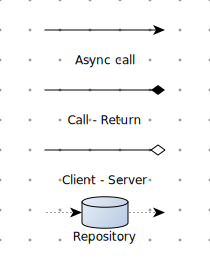
\includegraphics[scale=0.6]{graficos/call_reference.png}
	\caption{Referencia de conectores.}
\end{figure}

\subsubsection{Conectores no estandar}

\begin{itemize}
		%Completar con conectores no standard!
		%Agregar asi:
		\NonStandardConector{A non standard conector name}{A non standard conector description.}
\end{itemize}

\subsection{Subsistema de Query}

En el siguiente diagrama presenta el \textsf{Subsistema de Query} donde dada una consulta por productos (\textbf{query}) se arma la respuesta al usuario que realizó la consulta. En este diagrama se encuentran ejemplificados los \emph{casos de uso} 7, 8, 9, 10, 11 y 12.

\begin{figure}[H]
	\centering
	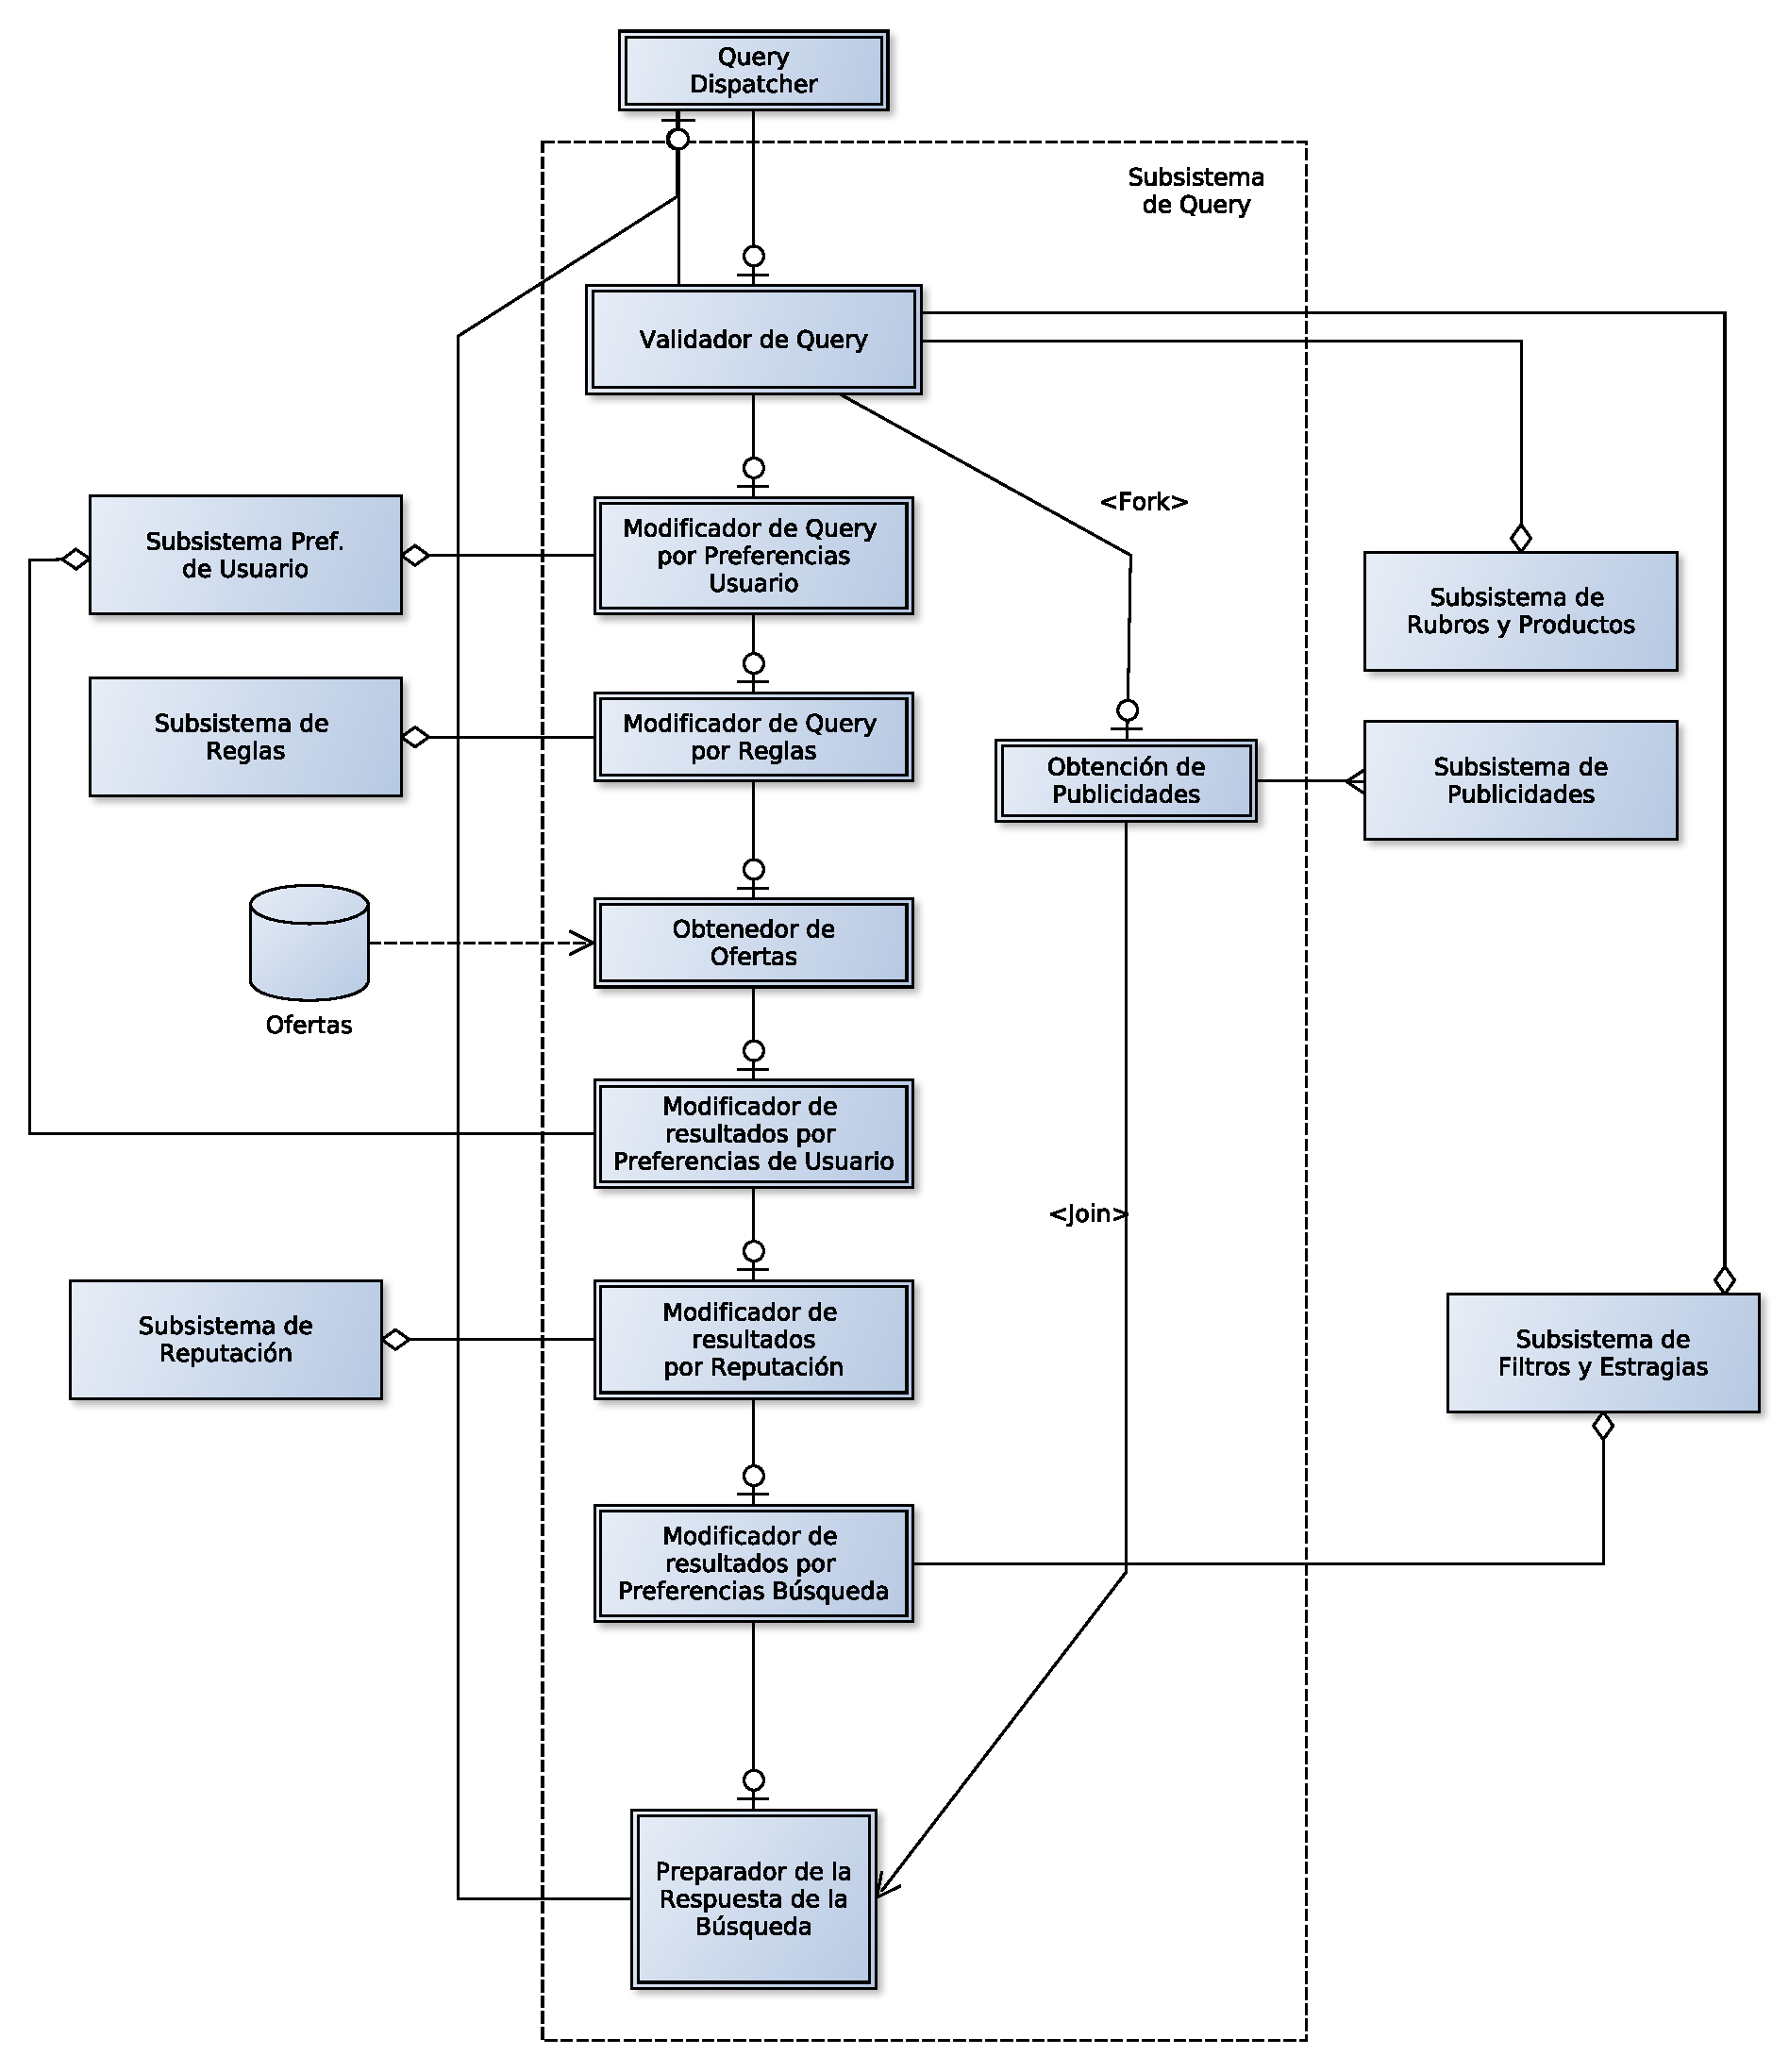
\includegraphics[width=\textwidth]{graficos/arch/subsistema_query.png}
	\caption{Diagrama arquitectónico con el detalle del \textsf{Subsistema de Query}.}
\end{figure}

\subsection{Interfaz movil}

\begin{figure}[H]
	\centering
	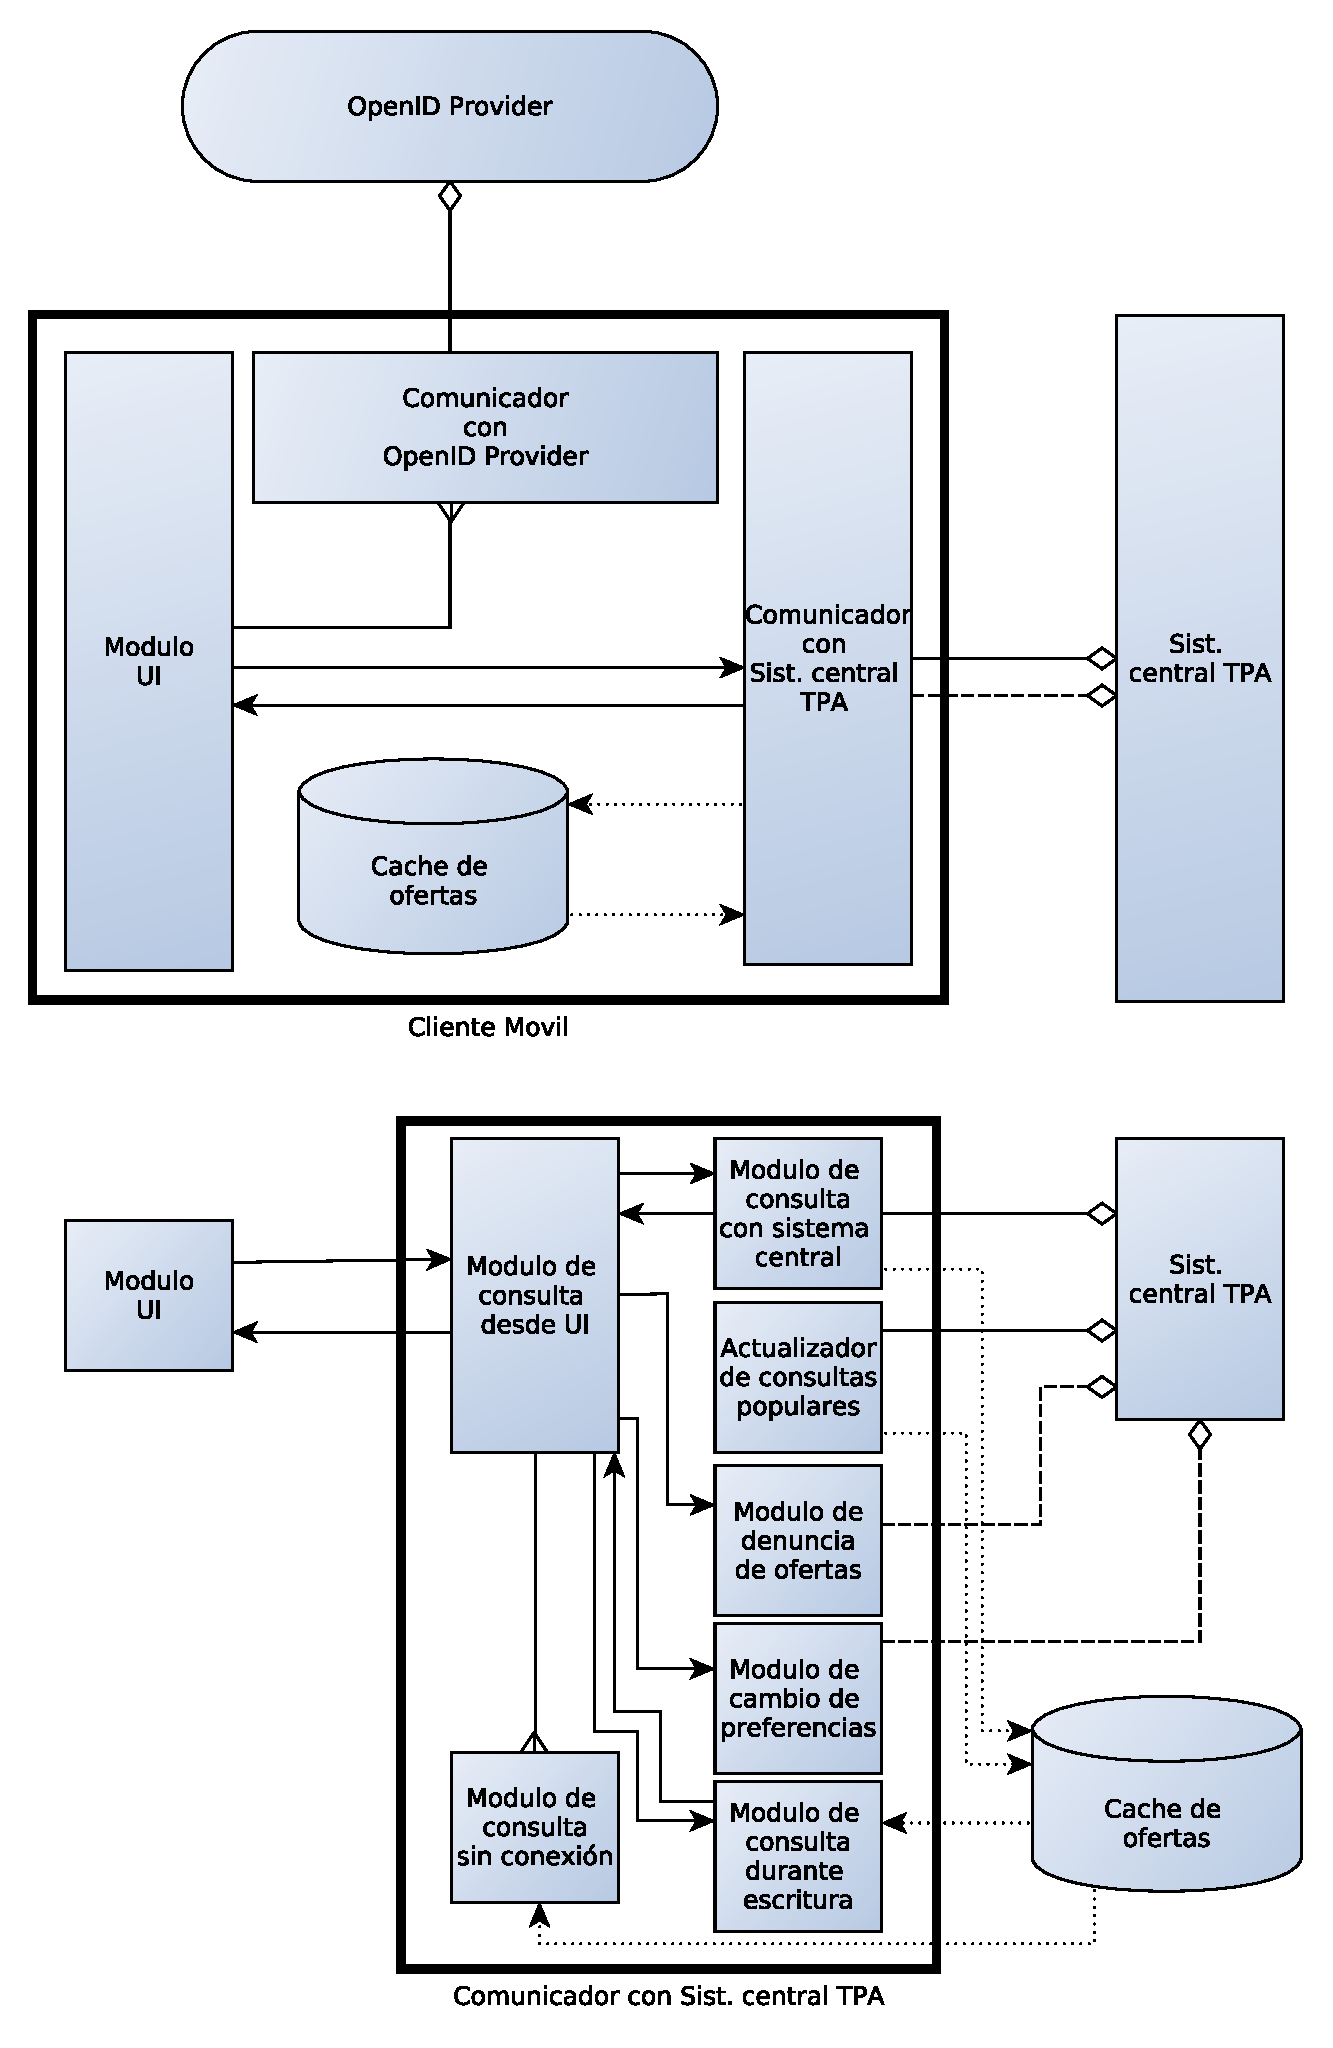
\includegraphics[width=\textwidth]{graficos/arch/Cliente_movil.png}
	\caption{Diagrama arquitectónico con el detalle del \textsf{Cliente movil}.}
\end{figure}


\section{Comparación}
	\label{sec:comparacion}

	\subsection{Comparación Metodologias agiles y Unified Process}

	Tanto \emph{Unified Process} como \emph{Scrum} son metodologias para el desarrollo de software, estas proponen un marco de trabajo para planificar y controlar distintas etapas en el desarrollo de software.

	Una caracteristica comun en ambas metodologias, es que siguen un proceso \emph{iterativo incremental}. Esto quiere decir que en ambas metodologias, el desarrollo del software se realiza en forma de iteraciones bien definidas. Una de las principales diferencias, encontradas durante la realización de los trabajos practicos de la materia, es que Unified Process organiza el desarrollo de software en distintas \emph{etapas} (\emph{inception, elaboration, construction} y \emph{transition}), cada etapa se diferencia de las otras en la actividad sobre la cual se pone enfasis. Sin embargo, en cada etapa se podrian realizar cada una de las posibles actividades (desarrollo, requerimientos, testing, etc...). Por otro lado, metodologias agiles como Scrum, no establecen nignuna distinción de etapas en el desarrollo.

	Esto se refleja en que para desarrollar la aplicación \emph{Precio Justo}, se partio de una escasa planeación sobre la construcción del software a desarrollar, en cambio, para \emph{Twitteando para ahorrar} se parte de un \emph{plan de iteraciones} y de una \emph{elaboración de la arquitectura} bien definida y documentada (si bien este plan y la arquitectura pueden estar sujetos a cambios).

	El desarrollo en Scrum, se centra en priorizar las funcionalidades que otorguen mas 'valor' al producto, esto se refleja en la idea de organizar las tareas a realizar en cada iteración en \emph{user stories}, una serie de historias, similares a casos de uso, contadas desde el punto de vista del usuario/product owner de la aplicación. En cambio, en Unified Process, las tareas a realizar en cada iteración estan son elegidas con el objetivo de reducir los riesgos. Para capturar las funcionalidades a implementar en cada iteración, Unified Process utiliza \emph{casos de uso}.

	De tener que escoger una metodologia para el desarrollo de software, nosotros creemos que \textbf{no} tiene sentido elegir de forma \emph{estricta} una unica metodologia. Nosotros proponemos utilizar ambas metodologias como un marco de ideas para construir una metodologia que se adapte de la mejor forma a nuestro equipo y al proyecto con el cual nos enfrentemos.

	Una de las diferencias que encontramos entre ambas metodologias, es que Scrum pide al final de cada iteración presentar un entregable, potencialmente listo a ser usado. De esta forma, se obtiene feedback temprano de los interesados en el proyecto. En cambio en UP, no necesariamente hace falta presentar un entregable con capacidad de funcionar.

	De ambas metodologias, las caracteristicas que mas nos gustaron son:

	\begin{itemize}
		\item El desarrollo \textbf{iterativo incremental}: El metodo iterativo incremental nos permite tener 'checkpoints' bien definidos, distribuidos mas o menos uniformemente en la linea de tiempo. Esto facilita el establecer objetivos chicos, alcanzables en el corto plazo, que ayudan a mantener al equipo focalizado. Ademas ayudan a obtener feedback de los interesados tempranamente. Esto ultimo es especialmente importante para descubrir si las expectativas de los interesados eran distintas a las del equipo de desarrollo, y permite tomar acciones rapidamente, para contrarrestar esta situación.

		\item De Scrum, la idea de \textbf{al final de cada iteración presentar un entregable}, para obtener feedback temprano de los usuarios. Sin embargo, en algunos casos es necesario ser flexible con esta condicion, en especial para proyectos grandes o que tienen poca interacción con el usuario, en las primeras iteraciones del proyecto.

		\item De Unified Process, el separar el desarrollo del sistema en \textbf{etapas}. Debido a que es esperable que en las primeras iteraciones, los esfuerzos se concentren en obtener requerimientos y planificar el proyecto, y que una vez que el proyecto se encuentra mas maduro, el foco se centre en programación, testing e integración.

		\item Las ideas de organizar el desarrollo en funcionalidades, representadas con \emph{user stories}, y decidir cuando implementar cada funcionalidad de acuerdo a una combinación de \textbf{business values} y minimización de \textbf{riesgos}. De esta forma, se intenta satisfacer cuanto antes los intereses de los stakeholders, y se intenta obtener feedback de ellos cuanto antes y al mismo tiempo, se tienen en cuenta los riesgos, que tienden a afectar fuertemente la arquitectura del sistema y de no tenerse en cuenta de forma temprana, podrian poner en riesgo el proyecto, o los tiempos planeados para completarlo.

		\item La elaboración detallada de la \textbf{arquitectura} como uno de los puntos centrales de la metodologia. Para, desde el inicio del proyecto, planificar el software para poder contrarrestar \emph{riesgos} y satisfacer los \emph{atributos de calidad} que restringen al proyecto. Ademas, el desarrollo de la arquitectura, suele dividir al sistema, en subsistemas mas pequeños, de los cuales es esperable que uno o dos desarrolladores puedan completar. Esto ayuda a la hora de asignar trabajo a los distintos miembros del equipo de desarrollo.

		\item De las metodologias agiles, uno de sus pautas claves, el \textbf{aceptar cambios} en los requerimientos e intentar adaptarse rapidamente a las circunstancias cambiantes que van surgiendo a lo largo del desarrollo de un proyecto.

		\item De Scrum, las \textbf{stand up meetings}, que ayudan a los distintos miembros del equipo a conocer en que componentes trabajan sus pares y permite comprender el estado de avance de la iteración en detalle. Esto favorece la sincronización de los distintos miembros del equipo.

	\end{itemize}

\subsection{Comparación 'programming in the small' y 'programming in the large'}

	\newcommand{\pil}{
		\emph{Programming in the large}
	}

	\newcommand{\pis}{
		\emph{Programming in the small}
	}

	\pil y \pis se utilizan para describir distintos enfoques al desarrollo de software.

	Tipicamente el termino \pis se utiliza para describir el desarrollo de un sistema compuesto por una cantidad relativamente pequeña de subsistemas que interactuan entre si. Estos sistemas suelen desarrollarse por equipos pequeños en una cantidad corta de tiempo.

	Por otra parte, \pil hace referencia al desarrollo de sistemas, compuestos por varios subsistemas. De forma que el proyecto es realizado por un gran numero de equipos, o por un equipo en una cantidad grande de tiempo.

	De esta forma, podriamos pensar a \pil como el desarrollar grandes proyectos de software y a \pis como el desarrollo de cada uno de sus subcomponentes mas pequeños, con tareas simples y bien definidas.

	La principal diferencia que pudimos encontrar entre ambas, es la rigurosidad con la cual se planifica cada una. En \pis, la planificación resulta minima, esto se debe en particular a que se desarrollan modulos pequeños en un periodo corto de tiempo. En cambio en \pil, el diseño del sistema surge de un analisis mas profundo de la problematica. \pil no solo maneja proyectos mas grandes, sino que un error de diseño en un la arquitectura del sistema, puede requerir cambios en varios modulos, que requieran una gran cantidad de horas/hombre. Esto ultimo se contrasta con un error de diseño introducido en un unico modulo, donde los cambios estan aislados.

	\nota{Despues si alguien puede abultar un poco mas}


\section{Casos de uso}
	\label{sec:cu}

	\begin{itemize}
\item
  Obteniendo informacion de internet \textbf{Descripción}: El sistema
  colecta la información de los distintos medios, la procesa, y la
  almacena para luego ser provista a los usuarios.
\item
  Se consulta información a travéz de el API publica.
  \textbf{Descripción}: Clientes externos pueden consultar a nuestro
  sistema por precios que recopilamos de distintos medios a través de un
  servicio público (API) ofrecido por nuestro sistema.
\item
  El usuario consulta precios a través de una interfaz amigable
  \textbf{Descripción}: El usuario accede a una aplicación de celular
  propia de \emph{twitteando para ahorrar} a través de la cual puede
  consultar por precios para distintos productos.
\item
  Se realizó una consulta por un producto, y el dispositivo sin tener
  conexión, logra responder la consulta de alguna forma medianamente
  satisfactoria. \textbf{Descripción}: El usuario accede a la aplicación
  de celular \emph{twitteando para ahorrar} sin tener conectividad a
  internet y recibe precios de los productos deseados y los relacionados
  a estos. La información provista al usuario podría estar limitada
  respecto de lo que vería si tuviera conectividad, pero esto no debería
  ser notado por el mismo.
\item
  ABM de rubros habilitados. \textbf{Descripción}: Ciertos usuarios
  particulares del sistema pueden acceder al mismo para agregar nuevos
  rubros o modificar o borrar existentes.
\item
  ABM de productos en un rubro. \textbf{Descripción}: Ciertos usuarios
  particulares del sistema pueden acceder al mismo para agregar nuevos
  productosi o modificar o borrar existentes. También pueden redefinir
  la pertenencia de un producto a uno o más rubros.
\item
  Si realizo una consulta por un producto A, obtengo ofertas de este
  producto. \textbf{Descripción}: El usuario consulta por un producto A
  dentro de los habilitados en algún rubro y recibe información de donde
  comprarlo y a qué precio.
\item
  Si realizo una consulta por un producto A y este no está se le informa
  al usuario. \textbf{Descripción}: El usuario consulta por un producto
  A que no está habilitado en ningún rubro y es informado que el sistema
  no posee información sobre donde comprar el mismo.
\item
  Si realizo una consulta por un producto A, y se considera que puede
  sustituirse por B, tambien se muestran ofertas de B.
  \textbf{Descripción}: El usuario consulta por un producto A dentro de
  los habilitados en algún rubro y se definió que puede sustituirse por
  el producto B, luego el usuario recibe información de donde comprar A
  y donde comprar B y a qué precio.
\item
  Si realizo una consulta por un producto A, que se considera asociado
  con B, tambien se muestran ofertas de B. \textbf{Descripción}: El
  usuario consulta por un producto A dentro de los habilitados en algún
  rubro y se definió que está asociado con el producto B, luego el
  usuario recibe información de donde comprar A y donde comprar B y a
  qué precio.
\item
  Si realizo una consulta por un producto A y soy un usuario
  autentificado, las ofertas recibidas se priorizan acorde a mis
  preferencias de confianza. \textbf{Descripción}: Dentro de las ofertas
  relacionadas al producto A que conoce el sistema, se mostrarán primero
  aquellas cuya fuente yo haya declarado de mayor confianza, luego las
  de fuentes con menor confianza y no se mostrará ninguna oferta cuya
  fuente declaré como no confiable.
\item
  Mostrando publicidades \textbf{Descripción}: Cuando el usuario utiliza
  la aplicación movil visualiza, aparte de los resultados de su
  consulta, propaganda de los spónsores de \emph{twitteando para
  ahorrar}.
\item
  Detectando ofertas falsas \textbf{Descripción}: Al recopilar datos de
  precios en internet, el sistema es capaz de detectar si la información
  es sospechosa y marcarla como tal, para futura revisión. Además el
  sistema recopila todas las evidencias encontradas para sospechar de
  los datos.
\item
  Siendo martes se publica un informe de ofertas falsas
  \textbf{Descripción}: Cada martes el sistema arma y publica un informe
  con los productos sobre los cuales se encontraron precios dudosos
  junto con la evidencia que genera la sospecha. Este informe debe estar
  disponible para revisión por usuarios externos selectos.
\item
  Se prepara un informe con las estadisticas de ofertas detectadas como
  falsas. \textbf{Descripción}: Al mismo tiempo que el usuario comienza
  a ingresar una consulta en la aplicación movil, la aplicación se
  anticipa a los deseos del usuario para mostrarle rápidamente precios
  de productos que podríán responder a la consulta que se está
  formulando.
\item
  El usuario se autentica con el sistema \textbf{Descripción}: El
  usuario de la aplicación movil puede utilizar alguna cuenta de un
  servicio asociado con OpenID (google, yahoo, facebook y otro) para
  autenticarse en la aplicación. A partir de ese momento la aplicación
  sabe quién es el usuario y puede utilizar la información que tiene del
  mismo para proveerle funcionalidades más avanzadas.
\item
  Un usuario autentificado puede votar por la validez de una oferta.
  \textbf{Descripción}: Un usuario ya autenticado en el sistema elije
  una oferta y la marca como válida o inválida. Esto afecta la
  reputación del usuario o fuente que dio origen a la oferta para
  facilitar la detección de ofertas sospechosas.
\end{itemize}


\end{document}
